% Copyright 2021 Fausto Spoto
%
% Licensed under the Apache License, Version 2.0 (the "License");
% you may not use this file except in compliance with the License.
% You may obtain a copy of the License at
%
%    http://www.apache.org/licenses/LICENSE-2.0
%
% Unless required by applicable law or agreed to in writing, software
% distributed under the License is distributed on an "AS IS" BASIS,
% WITHOUT WARRANTIES OR CONDITIONS OF ANY KIND, either express or implied.
% See the License for the specific language governing permissions and
% limitations under the License.

\documentclass[11pt]{beamer}  %% versione proiettore
%%\documentclass[11pt,handout]{beamer} %% versione stampa
\usepackage{slides}
\usepackage{mathtools}
\usepackage{relsize}
\usepackage[normalem]{ulem}

\mode<article>
{
  \usepackage{fullpage}
  \usepackage{hyperref}
}

\mode<presentation>
{
  \setbeamertemplate{background canvas}[vertical shading][bottom=red!10,top=blue!10]
  \usetheme{Course}
  \usefonttheme[onlysmall]{structurebold}
}

\subtitle{Trends in DLT 2021}
\title{Automatic\\ On-Chain Verification\\ of Java Smart Contracts}
\author{Luca Olivieri, \underline{Fausto Spoto} and Fabio Tagliaferro\\{\tiny Universit\`a di Verona, Italy}}
\date{April 2021}
\institute{Universit\`a di Verona, Italy}

\setbeamercovered{invisible}

\def\codesize{\smaller}
\def\<#1>{\codeid{#1}}
\newcommand{\codeid}[1]{\ifmmode{\mbox{\codesize\ttfamily{#1}}}\else{\codesize\ttfamily #1}\fi}

\begin{document}

\begin{frame}
  \titlepage
\end{frame}

\begin{frame}\frametitle{Smart contract verification by static analysis}

  \begin{greenbox}{Crowded world for Solidity}
    Echidna, Mythrill, MythX, Oyente, Securify, Slither, SmartCheck\ldots
  \end{greenbox}

  \bigskip

  They are all {\color{blue}off-chain} analyzers
  \begin{itemize}
  \item optional execution
  \item they do not protect the blockchain
  \item they may be expensive, since they are executed locally
  \end{itemize}

  \bigskip
  We want an {\color{blue}on-chain} analysis
  \begin{itemize}
  \item mandatory and automatic as an entry filter to the blockchain
  \item thus it protects the blockchain
  \item must be quick and cheap, since it is executed by all nodes of the blockchain
  \end{itemize}
\end{frame}

\begin{frame}
  \frametitle{Hotmoka}

  \begin{greenbox}{\url{https://github.com/Hotmoka/hotmoka}}
    An open-source implementation of a network of nodes:
    \begin{itemize}
    \item nodes of a blockchain
    \item IoT devices
    \item computers in the cloud
    \end{itemize}
    They execute smart contracts written in Takamaka (subset of Java)
  \end{greenbox}

  \bigskip
  \medskip

  \begin{greenbox}{Requests are OO-based}
    \begin{itemize}
    \item install a jar (zipped code archive)
    \item create an object
    \item call a method of an object
    \end{itemize}
  \end{greenbox}

\end{frame}

\begin{frame}\frametitle{We focus on Hotmoka nodes as Tendermint applications}

  \begin{center}
    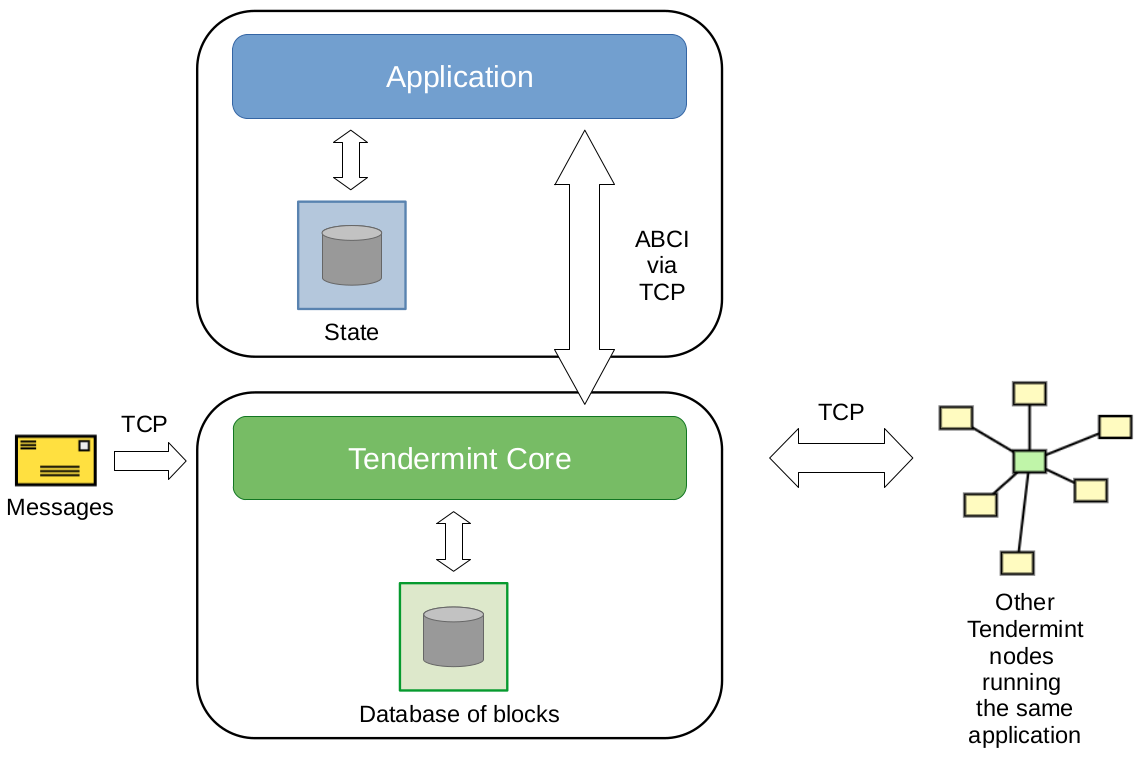
\includegraphics[scale=0.27,clip=false]{pictures/tendermint-databases.png}
  \end{center}
    
\end{frame}

\begin{frame}\frametitle{A set of verification rules}

  Hotmoka nodes perform a mandatory static analysis of the code
  sent along jar installation requests

  \begin{itemize}
  \item currently 26 checks are run, about the correct use of the syntactical
    features of Takamaka and to enforce determinism
  \item checks run at bytecode level, exploiting the BCEL library
  \item a single failure is enough to reject the code
  \item all nodes run the same rules
    $\Rightarrow$ verification rules are part of the consensus rules of the blockchain
  \item code that passes the verification step gets installed in the node
    and its future uses do not perform static analysis anymore
  \end{itemize}
\end{frame}

\begin{frame}[fragile]\frametitle{An insurance contract}

  \begin{greenbox}{The contract allows one to insure specific days of the year}
    If it rains on those days, one will get an indemnization larger than
    the cost of the insurance
    \begin{itemize}
    \item much larger in summer
    \item just a bit larger in winter
    \end{itemize}
  \end{greenbox}

  \medskip

  \begin{enumerate}
  \item construction, upon specification of the oracle:
    \[\<{\color{violet}@FromContract} {\color{airforceblue}@Payable} Insurance({\color{airforceblue}BigInteger amount}, Contract oracle)>\]
  \item purchase of an insurance for specific days:
    \[\<{\color{violet}@FromContract(PayableContract.class)} {\color{airforceblue}@Payable} void buy>\]
    \vspace*{-5ex}
    \[\<({\color{airforceblue}long amount}, int day, int month, int year, int duration)>\]
  \item notification of rain and indemnization:
    \[\<{\color{violet}@FromContract} void itRains()>\]
  \end{enumerate}
\end{frame}

\begin{frame}[fragile]\frametitle{An insurance contract}

  {\scriptsize\begin{semiverbatim}
public class Insurance extends {\color{blue}Contract} \{
  private final {\color{blue}Contract} oracle;
  private final {\color{blue}StorageSet}<InsuredDay> insuredDays = new {\color{blue}StorageTreeSet<>()};

  public {\color{violet}@FromContract} {\color{airforceblue}@Payable} Insurance({\color{airforceblue}BigInteger amount}, Contract oracle) \{
    this.oracle = oracle;
  \}

  {\color{red}// inner class}
  private static class InsuredDay extends {\color{blue}Storage} \{ {\color{red}/* shown later */} \}

  public {\color{violet}@FromContract(PayableContract.class)} {\color{airforceblue}@Payable} void buy
    ({\color{airforceblue}long amount}, int day, int month, int year, int duration) \{ {\color{red}/* shown later */} \}

  public {\color{violet}@FromContract} void itRains() \{ {\color{red}/* shown later */} \}
\}
  \end{semiverbatim}}

\end{frame}

\begin{frame}[fragile]\frametitle{The inner class}

\vspace{-1ex}
{\tiny\begin{semiverbatim}
private static class InsuredDay extends {\color{blue}Storage} \{
  private final PayableContract payer;
  private final long amount;
  private final int day, month, year;

  private InsuredDay(PayableContract payer, long amount, LocalDate when) \{
    this.payer = payer;
    this.amount = amount;
    this.day = when.getDayOfMonth();  this.month = when.getMonthValue();  this.year = when.getYear();
  \}

  private boolean isToday() \{
    return LocalDate.of(year, month, day).equals(today());
  \}

  private boolean isTodayOrBefore() \{
    return !LocalDate.of(year, month, day).isAfter(today());
  \}

  private static LocalDate today() \{
    Instant now = Instant.ofEpochMilli({\color{blue}Takamaka.now()});
    return LocalDate.ofInstant(now, ZoneId.of("Europe/Rome"));
  \}

  private long indemnization() \{
    switch (Season.now()) \{  {\color{red}// Season is an enumeration}
      case WINTER: return amount * 18 / 10; {\color{red}// 180%}
      case SPRING: return amount * 30 / 10; {\color{red}// 300%}
      case SUMMER: return amount * 50 / 10; {\color{red}// 500%}
      default /* FALL */ : return amount * 28 / 10; {\color{red}// 280%}
    \}
  \}
\}
\end{semiverbatim}}

\end{frame}

\begin{frame}[fragile]\frametitle{Buy an insurance}

{\scriptsize\begin{semiverbatim}
public final static long MIN = 1_000, MAX = 1_000_000_000;

public {\color{violet}@FromContract(PayableContract.class)} {\color{airforceblue}@Payable} void buy
    ({\color{airforceblue}long amount}, int day, int month, int year, int duration) \{

  {\color{armygreen}require(duration >= 1, "you must insure at least one day");
  require(duration <= 7, "you cannot insure more than a week");
  require(amount >= MIN * duration,
    () -> "we insure a single day for at least " + MIN + " units of coin");
  require(amount <= MAX * duration,
    () -> "we insure a single day for up to " + MAX + " units of coin");}

  // if the date is wrong, this generates an exception
  LocalDate start = LocalDate.of(year, month, day);

  PayableContract payer = (PayableContract) {\color{violet}caller()};
  for (int offset = 0; offset < duration; offset++)
    insuredDays.add(new InsuredDay
                    (payer, amount / duration, start.plusDays(offset)));
\}
\end{semiverbatim}}

\end{frame}

\begin{frame}[fragile]\frametitle{Pay the indemnization}

{\scriptsize\begin{semiverbatim}
public {\color{violet}@FromContract} void itRains() \{
  {\color{armygreen}require({\color{violet}caller()} == oracle, "only the oracle can call this method");}

  {\color{red}// pay who insured today}
  insuredDays.stream()
    .filter(InsuredDay::isToday)
    .forEachOrdered(insuredDay ->
          insuredDay.payer.{\color{blue}receive}(insuredDay.indemnization()));

  {\color{red}// clean-up the set of insured days}
  insuredDays.stream()
    .filter(InsuredDay::isTodayOrBefore)
    .forEachOrdered(insuredDays::remove);
\}
\end{semiverbatim}}

\end{frame}

%CLI install 251bfca0a37c0cc2611f3a5caee95fedb972e820609c6a0912d2527af53f59bb#0 target/insurance-0.0.1.jar --url ec2-54-194-239-91.eu-west-1.compute.amazonaws.com:8080
\begin{frame}[fragile]\frametitle{Installation of the jar into a remote node on AWS}

\begin{tt}mvn clean package\end{tt} $\Rightarrow$ generates \<target/insurance-0.0.1.jar>

\medskip

\begin{tt}
CLI install <payer> <jar>
\end{tt}

\bigskip

\begin{greenbox}{We use one of our accounts as payer}
{\scriptsize\begin{semiverbatim}
 {\color{red}CLI install
 \only<2>{payer}\only<3->{06aa6a1afabc82c7161ffcdc2391a2136101aaeb94f64edd53a1d0d1436d610e\#0}
 \only<4>{jar}\only<5->{target/insurance-0.0.1.jar}
 \onslide<6->{--url ec2-54-194-239-91.eu-west-1.compute.amazonaws.com:8080}}

\onslide<7->{Do you really want to spend up to 853900 gas units to install the jar [Y/N] Y

target/insurance-0.0.1.jar has been installed
at acb76103738dc7091c867c31bf6fb351f4d07b4bae1c7972e0e3bc3fcbf9e9c3
{\color{armygreen}Total gas consumed: 779976}
{\color{darkred}  for CPU: 255
  for RAM: 1326
  for storage: 778395
  for penalty: 0}}
\end{semiverbatim}}
\end{greenbox}

\end{frame}

%CLI create 251bfca0a37c0cc2611f3a5caee95fedb972e820609c6a0912d2527af53f59bb#0 it.univr.insurance.Insurance 1000000000000 06a080bbc4712862f875eefad00f43dee8f7daf98aec54c984d20861e3a219e6#0 --classpath acb76103738dc7091c867c31bf6fb351f4d07b4bae1c7972e0e3bc3fcbf9e9c3 --url ec2-54-194-239-91.eu-west-1.compute.amazonaws.com:8080
\begin{frame}[fragile]\frametitle{Creation of an instance of the \<Insurance> contract}

\begin{tt}
CLI create <payer> <class> <args> --classpath <jar>
\end{tt}

\bigskip

\begin{greenbox}{We use one of our accounts as payer and a previously existing oracle as argument
for the constructor}
{\scriptsize\begin{semiverbatim}
 {\color{red}CLI create
 \only<2>{payer}\only<3->{06aa6a1afabc82c7161ffcdc2391a2136101aaeb94f64edd53a1d0d1436d610e}
 \only<4>{class}\only<5->{it.univr.insurance.Insurance}
 \only<6>{args(amount, oracle)}\only<7->{1000000000000 06a080bbc4712862f875eefad00f43dee8f7daf98aec54c984d20861e3a219e6#0}
 \only<8>{--classpath jar}\only<9->{--classpath acb76103738dc7091c867c31bf6fb351f4d07b4bae1c7972e0e3bc3fcbf9e9c3}
 \only<10->{--url ec2-54-194-239-91.eu-west-1.compute.amazonaws.com:8080}}

\onslide<11->{Do you really want to spend up to 500000 gas units to call
public Insurance(java.math.BigInteger,io.takamaka.code.lang.Contract) ? [Y/N] Y

The new object has been allocated
at ffb8b8455979777e81708e3abac85b79ad455dfe8aa6a9849b11241c9c8ad7f7#0
{\color{armygreen}Total gas consumed: 47390}
{\color{darkred}  for CPU: 393
  for RAM: 1315
  for storage: 45682
  for penalty: 0}}
\end{semiverbatim}}
\end{greenbox}

\end{frame}

%CLI call 251bfca0a37c0cc2611f3a5caee95fedb972e820609c6a0912d2527af53f59bb#0 ffb8b8455979777e81708e3abac85b79ad455dfe8aa6a9849b11241c9c8ad7f7#0 buy 1000000 10 4 2021 2 --url ec2-54-194-239-91.eu-west-1.compute.amazonaws.com:8080
\begin{frame}[fragile]\frametitle{Let's insure next weekend against rain}

\begin{tt}
CLI call <payer> <receiver> <methodName> <args>
\end{tt}

\bigskip

\begin{greenbox}{We use one of our accounts as the buyer of the insurance}
{\scriptsize\begin{semiverbatim}
 {\color{red}CLI call
 \only<2>{payer}\only<3->{06aa6a1afabc82c7161ffcdc2391a2136101aaeb94f64edd53a1d0d1436d610e}
 \only<4>{receiver}\only<5->{ffb8b8455979777e81708e3abac85b79ad455dfe8aa6a9849b11241c9c8ad7f7#0}
 \only<6>{methodName}\only<7->{buy}
 \only<8>{args(amount, day, month, year, duration)}\only<9->{1000000 10 4 2021 2}
 \only<10->{--url ec2-54-194-239-91.eu-west-1.compute.amazonaws.com:8080}}

\onslide<11->{Do you really want to spend up to 500000 gas units to call
public void buy(long,int,int,int,int) ? [Y/N] Y

{\color{armygreen}Total gas consumed: 12340}
{\color{darkred}  for CPU: 1587
  for RAM: 2943
  for storage: 7810
  for penalty: 0}}
\end{semiverbatim}}
\end{greenbox}

\end{frame}

%CLI install 251bfca0a37c0cc2611f3a5caee95fedb972e820609c6a0912d2527af53f59bb#0 target/insurance-0.0.1.jar --url ec2-54-194-239-91.eu-west-1.compute.amazonaws.com:8080
\begin{frame}[fragile]\frametitle{On-chain verification: incorrect use of annotations}

  \begin{redbox}{Assume that the programmer forgets the \<FromContract> annotation in \<buy>}
  \<public {\color{blue}\sout{@FromContract(PayableContract.class)}} @Payable void buy
  (long amount, int day, int month, int year, int duration)>
  \end{redbox}\pause

  \begin{tt}mvn clean package\end{tt} $\Rightarrow$ regenerates \<target/insurance-0.0.1.jar>\pause

\medskip

\begin{greenbox}{Let's try to install this version of the jar}
{\scriptsize\begin{semiverbatim}
 {\color{red}CLI install
 06aa6a1afabc82c7161ffcdc2391a2136101aaeb94f64edd53a1d0d1436d610e\#0
 target/insurance-0.0.1.jar
 --url ec2-54-194-239-91.eu-west-1.compute.amazonaws.com:8080}\pause

Do you really want to spend up to 852500 gas units to install the jar [Y/N] Y
{\color{armygreen}Total gas consumed: 852500}
{\color{darkred}  for CPU: 255
  for RAM: 1326
  for storage: 381762
  for penalty: 469157     !!!!!!!}
io.hotmoka.beans.TransactionException:
io.takamaka.code.verification.VerificationException:
{\color{red}it/univr/insurance/Insurance.java method buy:
@Payable can only be applied to a @FromContract method or constructor}
\end{semiverbatim}}
\end{greenbox}

\end{frame}

%CLI install 251bfca0a37c0cc2611f3a5caee95fedb972e820609c6a0912d2527af53f59bb#0 target/insurance-0.0.1.jar --url ec2-54-194-239-91.eu-west-1.compute.amazonaws.com:8080
\begin{frame}[fragile]\frametitle{On-chain verification: potential non-determinism}

  \begin{redbox}{Assume to use \<forEach> instead of \<forEachOrdered> in \<itRains>}
\<insuredDays.stream().filter(InsuredDay::isToday).{\color{blue}forEach\sout{Ordered}}(...);>
  \end{redbox}\pause

  \begin{tt}mvn clean package\end{tt} $\Rightarrow$ regenerates \<target/insurance-0.0.1.jar>\pause

\medskip

\begin{greenbox}{Let's try to install this version of the jar}
{\scriptsize\begin{semiverbatim}
 {\color{red}CLI install
 06aa6a1afabc82c7161ffcdc2391a2136101aaeb94f64edd53a1d0d1436d610e\#0
 target/insurance-0.0.1.jar
 --url ec2-54-194-239-91.eu-west-1.compute.amazonaws.com:8080}\pause

Do you really want to spend up to 852500 gas units to install the jar [Y/N] Y

{\color{armygreen}Total gas consumed: 853700}
{\color{darkred}  for CPU: 255
  for RAM: 1326
  for storage: 382362
  for penalty: 469757     !!!!!!!}
io.hotmoka.beans.TransactionException:
io.takamaka.code.verification.VerificationException:
{\color{red}it/univr/insurance/Insurance.java:95:
illegal call to non-white-listed method java.util.stream.Stream.forEach}
\end{semiverbatim}}
\end{greenbox}

\end{frame}

%CLI verify target/insurance-0.0.1.jar --libs io-takamaka-code-1.0.0.jar
\begin{frame}[fragile]\frametitle{Off-chain verification}

Using the blockchain as a debugger is very expensive\ldots

\medskip
\begin{tt}
CLI verify <jar> --libs dependencies
\end{tt}\pause

\medskip

\begin{greenbox}{We verify the jar off-chain, to find all errors}
{\scriptsize\begin{semiverbatim}
 {\color{red}CLI verify
 \only<3>{jar}\only<4->{target/insurance-0.0.1.jar}
 \only<5>{--libs dependencies}\only<6->{--libs io-takamaka-code-1.0.0.jar}}
\onslide<7->{
{\color{red}
it/univr/insurance/Insurance.java method buy:
  @Payable can only be applied to a @FromContract method or constructor
it/univr/insurance/Insurance.java:46:
  caller() can only be used inside a @FromContract method or constructor
it/univr/insurance/Insurance.java:95:
  illegal call to non-white-listed method java.util.stream.Stream.forEach
it/univr/insurance/Insurance.java:99:
  illegal call to non-white-listed method java.util.stream.Stream.forEach
}}
\end{semiverbatim}}
\end{greenbox}

\end{frame}

\begin{frame}\frametitle{Verification is currently very cheap}

  \begin{itemize}
  \item correct use of Takamaka annotations
  \item determinism (hence no finalizers and no reflection)
  \item correct types for storage classes
  \item no \emph{unusual} bytecodes (reassignment of local 0, \<jsr>, \<ret>\ldots)
  \item no catch of unchecked exceptions
  \item no static fields (almost)
  \item no native code
  \end{itemize}

  \medskip

  \begin{greenbox}{The time spent for static analysis is irrelevant}
    We have written a stress test whose execution time passes from 157s (without verification)
    to 158s (with verification)
  \end{greenbox}

  \medskip

  \begin{center}
    Things would change with more expensive static analyses!
  \end{center}
  
\end{frame}

\begin{frame}[fragile]\frametitle{Can you prove that there is no overflow and no division by zero here? ({\color{red}Hotmoka currently does not check it})}

{\scriptsize\begin{semiverbatim}
public final static long MIN = 1_000, MAX = 1_000_000_000;

public {\color{violet}@FromContract(PayableContract.class)} {\color{airforceblue}@Payable} void buy
    ({\color{airforceblue}long amount}, int day, int month, int year, int duration) \{

  {\color{armygreen}require(duration >= 1, "you must insure at least one day");
  require(duration <= 7, "you cannot insure more than a week");
  require(amount >= \fbox{MIN * duration},
    () -> "we insure a single day for at least " + MIN + " units of coin");
  require(amount <= \fbox{MAX * duration},
    () -> "we insure a single day for up to " + MAX + " units of coin");}

  LocalDate start = LocalDate.of(year, month, day);
  PayableContract payer = (PayableContract) {\color{violet}caller()};
  for (int offset = 0; offset < duration; \fbox{offset++})
    insuredDays.add(new InsuredDay
                    (payer, \fbox{amount / duration}, start.plusDays(offset)));
\}
\end{semiverbatim}}

\vspace*{-2ex}
\begin{center}
  {\color{red}Can you prove the same for the inner class \<InsuredDay>}?

  (spoiler: yes, but it is very hard for an automatic tool)
\end{center}

\end{frame}

\begin{frame}\frametitle{Upgrading the verification rules}

  \begin{greenbox}{A realistic scenario, triggered by a poll among the validators}
    \begin{itemize}
    \item more precise verification rules
    \item more verification rules
    \end{itemize}
  \end{greenbox}

  \bigskip

  \begin{greenbox}{Code already verified with rules version $n$ is reverified
      when switching to rules version $n+1$}
    \begin{itemize}
    \item {\color{red}is this the right choice?}
    \item reverification runs on-demand (the first time, and only the first, that a jar is used after the switch)
    \item the fact that $80\%$ of transactions
      involves only $0.05\%$ of all smart contracts (data from Ethereum) justifies this
      lazy approach
    \item code that does not satisfy rules version $n+1$ cannot be run and will
      never be reactivated in the future
      \begin{itemize}
      \item {\color{red}is this the right choice?}
      \item {\color{red}what about the balance of contracts that get disabled?}
      \end{itemize}
    \end{itemize}
  \end{greenbox}

\end{frame}

\begin{frame}{}

  \begin{center}
    {\Huge Thanks!}
  \end{center}

  \bigskip
  \bigskip

  \begin{center}
    
\includegraphics[scale=0.12,clip=false]{pictures/hotmoka_logo.png}

    {\scriptsize
    free, simple, open-source

    \url{https://github.com/Hotmoka/hotmoka}}

  \end{center}

  \bigskip
  \bigskip
  {\tiny
  L.\ Olivieri, F.\ Spoto and F.\ Tagliaferro: \emph{On-Chain Smart Contract Verification over Tendermint}, WTSC 2021, to appear\\\mbox{}\\

  F.\ Spoto: \emph{Enforcing Determinism of Java Smart Contracts}, WTSC 2020, LNCS 12063

  F.\ Spoto: \emph{A Java Framework for Smart Contracts}, WTSC 2019, LNCS 11599}
\end{frame}

\end{document}
